% ---------------------------------------------------------------
% Preamble
% ---------------------------------------------------------------
%\documentclass[a4paper,fleqn,longmktitle]{cas-sc}
\documentclass[a4paper,fleqn]{cas-dc}
%\documentclass[a4paper]{cas-dc}
%\documentclass[a4paper]{cas-sc}
% ---------------------------------------------------------------
% Make margins bigger to fit annotations. Use 1, 2 and 3. TO be removed later
%\paperwidth=\dimexpr \paperwidth + 6cm\relax
%\oddsidemargin=\dimexpr\oddsidemargin + 3cm\relax
%\evensidemargin=\dimexpr\evensidemargin + 3cm\relax
%\marginparwidth=\dimexpr \marginparwidth + 3cm\relax
% -------------------------------------------------------------------- 
% Packages
% --------------------------------------------------------------------
% Figure packages
\usepackage{graphicx}
\usepackage{float}
\restylefloat{table}
\usepackage{adjustbox}
% Text, input, formatting, and language-related packages
\usepackage[T1]{fontenc}
\usepackage{subcaption}

\usepackage{csvsimple}

% TODO package
\usepackage[bordercolor=gray!20,backgroundcolor=blue!10,linecolor=black,textsize=footnotesize,textwidth=1in]{todonotes}
\setlength{\marginparwidth}{1in}
% \usepackage[utf8]{inputenc}
% \usepackage[nomath]{lmodern}

% Margin and formatting specifications
%\usepackage[authoryear]{natbib}
\usepackage[sort]{natbib}
\setcitestyle{square,numbers}

 %\bibliographystyle{cas-model2-names}

\usepackage{setspace}
\usepackage{subfiles} % Best loaded last in the preamble

% \usepackage[authoryear,longnamesfirst]{natbib}

% Math packages
\usepackage{amsmath, amsthm, amssymb, amsfonts, bm, nccmath, mathdots, mathtools, bigints, ulem}

\usepackage{tikz}
\usepackage{pgfplots}
\usetikzlibrary{shapes.geometric,angles,quotes,calc}

\usepackage{placeins}

\usepackage[final]{pdfpages}

\usepackage{numprint}

% --------------------------------------------------------------------
% Packages Configurations
\usepackage{enumitem}
% --------------------------------------------------------------------
% (General) General configurations and fixes
\AtBeginDocument{\setlength{\FullWidth}{\textwidth}}	% Solves els-cas caption positioning issue
\setlength{\parindent}{20pt}
%\doublespacing
% --------------------------------------------------------------------
% Other Definitions
% --------------------------------------------------------------------
\graphicspath{{Figures/}}
% --------------------------------------------------------------------
% Environments
% --------------------------------------------------------------------
% ...

% --------------------------------------------------------------------
% Commands
% --------------------------------------------------------------------

% ==============================================================
% ========================== DOCUMENT ==========================
% ==============================================================
\begin{document} 
%  --------------------------------------------------------------------

% ===================================================
% METADATA
% ===================================================
\title[mode=title]{Supercritical fluid extraction of essential oil from chamomile flowers: modelling, and parameter estimation}                      
\shorttitle{Supercritical fluid extraction of essential oil from chamomile flowers: modelling, and parameter estimation}

\shortauthors{OS, PO}

\author[1]{Oliwer Sliczniuk}[orcid=0000-0003-2593-5956]
\ead{oliwer.sliczniuk@aalto.fi}
\cormark[1]
\credit{a}

\author[1]{Pekka Oinas}[orcid=0000-0002-0183-5558]
\credit{b}

\address[1]{Aalto University, School of Chemical Engineering, Espoo, 02150, Finland}
%\address[2]{2}

\cortext[cor1]{Corresponding author}

% ===================================================
% ABSTRACT
% ===================================================
\begin{abstract}
This study investigated the supercritical extraction process of chamomile extract from chamomile flowers. A distributed-parameter model describes the fluid-solid extraction process. The concept of quasi-one-dimensional flow is applied to reduce the number of spatial dimensions. The flow is assumed to be uniform across any cross-section, although the area available for the fluid phase can vary along the extractor. The physical properties of the solvent are estimated from the Peng-Robinson equation of state. Model parameters, including the partition factor, internal diffusion coefficient, axial diffusion coefficient, and decaying factor, were determined through maximum likelihood estimation based on experimental data, with the assumption of normally distributed errors. A set of laboratory experiments was performed under multiple constant operating conditions: $30 - 40^\circ C$, $100 - 200$ bar, and $3.33-6.67 \times 10^{-5}$ kg/s. 

\end{abstract}

\begin{keywords}
Supercritical extraction \sep Parameter estimation \sep Mathematical modelling
\end{keywords}

% ===================================================
% TITLE
% ===================================================
\maketitle

% ===================================================
% Section: Introduction
% ===================================================\section{Introduction}

\section{Introduction}
\subfile{Sections/introduction_imp}

\section{Materials and methods} \label{CH: Materials and methods}

%\subsection{Supercritical fluids} \label{CH: Thermodynamic}
%\subfile{Sections/Thermo_imp}

\subsection{Governing equations} \label{CH:Governing_equations_chapter}
	The governing equations for quasi-one-dimensional compressible flow in Cartesian coordinates are detailed in Appendix \ref{CH: Gouverning equations} and are based on the foundational work by \citet{Anderson1995}. Quasi-one-dimensional flow refers to a fluid flow scenario where it's assumed that flow properties are uniformly distributed across any given cross-section. This simplification is typically applied in situations where the flow channel's cross-sectional area changes, such as through irregular shapes or partial fillings of an extractor. In these instances, the flow is considered quasi-one-dimensional because it's presumed that velocity and other flow properties change solely along the flow direction.
	
	The set of quasi-one-dimensional compressible Navier-Stokes equations in Cartesian coordinates are described by Equations \ref{EQ: CompressibleEuler_1} through \ref{EQ: CompressibleEuler_3}. The formulation of these equations is elaborated upon in Appendix \ref{CH: Gouverning equations}, providing a mathematical foundation for analyzing flow dynamics under the assumed conditions.

{\footnotesize
	\begin{align}
		\label{EQ: CompressibleEuler_1}
		\cfrac{\partial \left( {\color{black}\rho_f} {\color{black}A_f}(z) \right) }{\partial t} + \cfrac{\partial \left( {\color{black}\rho_f} {\color{black}A_f}(z) v \right)}{\partial z} &= 0 \\
		\cfrac{\partial \left( {\color{black}\rho_f} v {\color{black}A_f}(z) \right) }{\partial t} + \cfrac{\partial \left( {\color{black}\rho_f} {\color{black}A_f}(z) v^2 \right)}{\partial z} &= -{\color{black}A_f}(z) \cfrac{\partial {\color{black}P}}{\partial z} \label{EQ: CompressibleEuler_2} \\
		\cfrac{\partial \left( {\color{black}\rho_f} {\color{black}e} {\color{black}A_f}(z) \right) }{\partial t} + \cfrac{\partial \left( {\color{black}\rho_f} {\color{black}A_f}(z) v {\color{black}e}\right)}{\partial z} &= -{\color{black}P}\cfrac{\left( {\color{black}A_f}(z) v \right)}{\partial z} + \cfrac{\partial}{\partial z} \left( k \cfrac{\partial {\color{black}T}}{\partial z} \right)   
		\label{EQ: CompressibleEuler_3}
	\end{align}  
}

where ${\color{black}\rho_f}$ is the density of the fluid, ${\color{black}A_f}(z)$ is the function which describe change of the cross-section, $v$ is the velocity, ${\color{black}P}$ is the total pressure, ${\color{black}e}$ is the internal energy of the fluid, $t$ is time and $z$ is the spacial direction.

Based on governing equations, the small discontinuity (defined as $\delta$) in flow properties, shown in Figure \ref{fig: Discontinuity_slow_flow}, can be analysed. The analysis follows the work of \citet{Schreier1982}.

\begin{figure}[!h]
	\centering
	\resizebox{0.95\columnwidth}{!}{%
		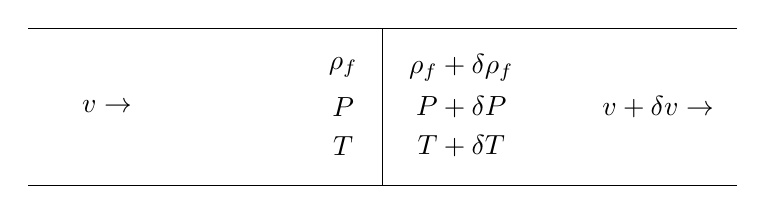
\begin{tikzpicture}[]
			\draw (0,2) -- (9,2);	% Top line
			\draw (0,0) -- (9,0); 	% Bottom line
			\draw (4.5,0) -- (4.5,2); 	% Bottom line
			\node at (4,1.5) {${\color{black}\rho_f}$};
			\node at (5.5,1.5) {${\color{black}\rho_f}+\delta{\color{black}\rho_f}$};
			\node at (4,1.0) {${\color{black}P}$};
			\node at (5.5,1.0) {${\color{black}P}+\delta {\color{black}P}$};
			\node at (4,0.5) {${\color{black}T}$};
			\node at (5.5,0.5) {${\color{black}T}+\delta {\color{black}T}$};
			\node at (1,1.0) {$v \rightarrow$};
			\node at (8,1.0) {$v + \delta v \rightarrow$};
	\end{tikzpicture} }
	\caption{Small discontinuity in one-dimensional flow}
	\label{fig: Discontinuity_slow_flow}
\end{figure} 

The discontinuity is presumed to be at rest relative, and the balance equations become		

{\footnotesize
	\begin{align*}
		&{\color{black}\rho_f} \delta v + v \delta {\color{black}\rho_f} + \delta {\color{black}\rho_f} \delta v = 0 \\
		&\delta {\color{black}P} = \delta v \delta {\color{black}\rho_f}
	\end{align*}
}

These relations are equally valid if both regions are separated by a region of finite width rather than a discontinuity. 

{\footnotesize
	\begin{equation*}
		\lim_{{\color{black}\rho_f} v \rightarrow 0} {\color{black}\rho_f} \delta v + v \delta {\color{black}\rho_f} + \delta {\color{black}\rho_f} \delta v = 0 / \delta {\color{black}\rho_f} \rightarrow \cfrac{d v}{d {\color{black}\rho_f}} = - \cfrac{v}{{\color{black}\rho_f}}
	\end{equation*}
}

By combining the momentum equation with the above equation, we get

{\footnotesize
	\begin{equation} \label{EQ: Pressure_Velocity}
		\cfrac{d v}{d {\color{black}\rho_f}} = - \cfrac{d v}{d{\color{black}P}} \cfrac{d {\color{black}P}}{d {\color{black}\rho_f}} = -\cfrac{1}{\rho v} \cfrac{d{\color{black}P}}{d{\color{black}\rho_f}} = -\cfrac{v}{{\color{black}\rho_f}}
	\end{equation}
}

Suppose the flow is presumed to be isentropic, $d{\color{black}P}/d{\color{black}\rho_f} = c^2$, so $v^2=c^2$, where $c$ is the speed of sound. This can be interpreted as a small pressure wave propagating with the speed of sound relative to the flow. If the flow velocity is relatively low, all pressure changes are hydrodynamic (due to velocity motion) rather than thermodynamic, which leads to $\partial {\color{black}\rho_f} / \partial {\color{black}P} \approx 0$. The small changes in pressure due to flow velocity changes do not change the density. 

The low Mach number condition leads to the incompressible condition: $\nabla \cdot u =0$, which is valid for constant density (strict incompressible) or varying density flow. The restraint allows for the removal of acoustic waves, but also allows for large perturbations in density and/or temperature. The assumption is that the flow remains within a Mach number limit (usually less than 0.3) for any solution using such a constraint to be valid. In the 1-D case, the incompressibility condition becomes $\frac{du}{dz} = 0$, so the fluid velocity is constant.

\subsection{Extraction model} \label{CH: Extraction_model}
\subfile{Sections/Model}

\subsection{Parameter estimation} \label{CH: Parameter_estimation}
\subfile{Sections/Parameter_estimation}

\begin{figure*}[!b]
	\centering
	\begin{subfigure}{0.3\textwidth}
		\centering
		\includegraphics[trim = 0.0cm 0.0cm 0.0cm 0.0cm,clip, width=\textwidth]{/Results_estimation/Parameter_Space_Linear_Dataset_1.png}
		\caption{Parameter space: the linear kinetic model}
		\label{fig: Fit_1_linear}
	\end{subfigure}
	\hfill
	\begin{subfigure}{0.3\textwidth}
		\centering
		\includegraphics[trim = 0.0cm 0.0cm 0.0cm 0.0cm,clip, width=\textwidth]{/Results_estimation/Parameter_Space_Di_Dx_Dataset_1.png}
		\caption{Parameter space: the reduced linear kinetic model with axial diffusion}
		\label{fig: Fit_1_Di_Dx}
	\end{subfigure}
	\hfill
	\begin{subfigure}{0.3\textwidth}
		\centering
		\includegraphics[trim = 0.0cm 0.0cm 0.0cm 0.0cm,clip, width=\textwidth]{/Results_estimation/Parameter_space_Di_Gamma_dataset_1_org.png}
		\caption{Parameter space: the modified model}
		\label{fig: Fit_1_Di_Gamma}
	\end{subfigure}
	\caption{Parameter estimation results for experiment 1}
	%\label{fig: Fit_Di_Gamma}
\end{figure*}

\subsection{Experimental work}
\subfile{Sections/Experiments}

\section{Results}
\subfile{Sections/Results_Chamomile}

\section{Conclusions} \label{CH: Conclusion}

\begin{figure*}[!h]
	\centering
	\begin{subfigure}{0.3\textwidth}
		\centering
		\includegraphics[trim = 0.0cm 0.0cm 0.0cm 0.0cm,clip, width=\textwidth]{/Results_estimation/Fit_Di_Gamma_1_4_correlation.png}
		\caption{Results of parameter estimation for experiments at $6.67\times 10^{-5}$ [kg/s]}% and temperature of 40 $[^\circ C]$}
		\label{fig: Fit_1_4_Di_Gamma_correlation}
	\end{subfigure}
	\hfill
	\begin{subfigure}{0.3\textwidth}
		\centering
		\includegraphics[trim = 0.0cm 0.0cm 0.0cm 0.0cm,clip, width=\textwidth]{/Results_estimation/Fit_Di_Gamma_5_8_correlation.png}
		\caption{Results of parameter estimation for experiments at $6.67\times 10^{-5}$ [kg/s]}% and temperature of 30 $[^\circ C]$}
		\label{fig: Fit_5_8_Di_Gamma_correlation}
	\end{subfigure}
	\hfill
	\begin{subfigure}{0.3\textwidth}
		\centering
		\includegraphics[trim = 0.0cm 0.0cm 0.0cm 0.0cm,clip, width=\textwidth]{/Results_estimation/Fit_Di_Gamma_9_12_correlation.png}
		\caption{Results of parameter estimation for experiments at $3.33\times 10^{-5}$ [kg/s]}
		\label{fig: Fit_9_12_Di_Gamma_correlation}
	\end{subfigure}
	\caption{Parameter estimation results}
	\label{fig: Fit_Di_Gamma_correlation}
\end{figure*}

The article presents a comprehensive study on supercritical fluid extraction of essential oil from chamomile flowers, focusing on developing and applying a distributed-parameter model to describe the fluid-solid extraction process. By employing the concept of quasi-one-dimensional flow, the study simplifies the spatial dimensions of the extraction process, ensuring uniform flow across any cross-section while allowing for variations in the area available for the fluid phase. The physical properties of the solvent are estimated using the Peng-Robinson equation of state, and key model parameters are determined through maximum likelihood estimation based on experimental data, considering normally distributed errors.

Laboratory experiments were conducted under various conditions to validate the model. The model parameters, such as partition factor, internal diffusion coefficient, axial diffusion coefficient, and decaying factor, were determined through maximum likelihood estimation based on experimental data. The parameter space exploration revealed that while some parameters could be determined with a high degree of confidence, others, like the axial diffusion coefficient, had a low impact on the model's output. The identification of the low-impact parameters leads to model reduction

This work introduced a set of correlations to find a general relationship between parameters and the independent variables, which can be determined by operating conditions. The obtained correlations were introduced into the model and tested against the dataset. The results show good agreement between the simulation results and all the data points.

The presented model can be further used with the presented correlations to introduce an extraction model with dynamically changing operating conditions for multiple purposes, such as yield maximisation, techno-economic analysis, or optimal experiments design.

% ===================================================
% Bibliography
% ===================================================
%% Loading bibliography style file
%\clearpage
%\bibliographystyle{model1-num-names}
\bibliographystyle{unsrtnat}
\bibliography{mybibfile}

\clearpage \appendix \label{appendix}
\section{Appendix} 

\subsection{Governing equations}
\subfile{Sections/Gouverning_equation_derivation}

\subsection{Thermodynamic}
\subfile{Sections/Qubic_EOS} \label{CH: EOS}


\subsection{Cardano's Formula} \label{CH: Cardano}
\subfile{Sections/Cardano}

%\subsection{Initial and boundary conditions} \label{CH: IC_BC}
%\subfile{Sections/IC_BC}

\subsection{Maximum likelihood} \label{CH: ML}
\subfile{Sections/Likelihood}

%\subsection{Solid density measurement} \label{CH: Solid_Density_Measurment}

%Figure \ref{fig:density_cal} shows results of density measurement performed with pycnometer.

%\begin{figure}[!h]
%	\centering 
%	\includegraphics[trim=2cm 6cm 4cm 0cm, clip,width=\columnwidth]{Sections/ultraReportT5.pdf}
%	\caption{The result of solid density measurement}
%	\label{fig:density_cal}
%\end{figure}

%{\footnotesize
%	\begin{equation*}
%		\rho_s^{ave} = \frac{1.2585+1.2582+1.2561+1.2546+1.2555}{5} = 1.25658 [g/cc]
%	\end{equation*}
%}

%\subsection{Porosity calculations} \label{CH: Porosity}
%\subfile{Sections/Porosity}

\end{document}